% Created 2022-10-06 jue 13:22
% Intended LaTeX compiler: pdflatex
\documentclass[12pt]{article}
\usepackage[utf8]{inputenc}
\usepackage[T1]{fontenc}
\usepackage{graphicx}
\usepackage{grffile}
\usepackage{longtable}
\usepackage{wrapfig}
\usepackage{rotating}
\usepackage[normalem]{ulem}
\usepackage{amsmath}
\usepackage{textcomp}
\usepackage{amssymb}
\usepackage{capt-of}
\usepackage{hyperref}
\usepackage[spanish]{babel}
\usepackage{graphicx,geometry}
\geometry{ a4paper, left=1in, right=1in, top=1in, bottom=1in }
\renewcommand\familydefault{\sfdefault}
\usepackage{sectsty}
\sectionfont{\normalfont\Large }
\subsectionfont{\normalfont\normalsize}
\usepackage{tabularx}
\usepackage{listings}
\lstdefinestyle{mystyle}{
numbers=left,
showspaces=false,
frame=leftline,
showspaces=false,
showstringspaces=false,
showtabs=false,
numberstyle=\tiny,
}
\lstset{
style=mystyle,
literate={á}{{\'a}}1
{é}{{\'e}}1
{í}{{\'{\i}}}1
{ó}{{\'o}}1
{ú}{{\'u}}1
{Á}{{\'A}}1
{É}{{\'E}}1
{Í}{{\'I}}1
{Ó}{{\'O}}1
{Ú}{{\'U}}1
{ü}{{\"u}}1
{Ü}{{\"U}}1
{ñ}{{\~n}}1
{Ñ}{{\~N}}1
{¿}{{?``}}1
{¡}{{!``}}1
}
\makeatletter
\usepackage{fancyhdr}
\pagestyle{fancy}
\usepackage{mdframed}
\BeforeBeginEnvironment{minted}{\begin{mdframed}}
\AfterEndEnvironment{minted}{\end{mdframed}}
\author{Luis Eduardo Galindo Amaya (1274895)}
\date{06-10-2022}
\title{Laboratorio 1 - Correlación}
\hypersetup{
 pdfauthor={Luis Eduardo Galindo Amaya (1274895)},
 pdftitle={Laboratorio 1 - Correlación},
 pdfkeywords={},
 pdfsubject={},
 pdfcreator={Emacs 26.3 (Org mode 9.1.9)}, 
 pdflang={Spanish}}
\begin{document}


\newcommand{\docente}{Olivia Mendoza Duarte}
\newcommand{\asignatura}{Estadística Avanzada}
\newcommand{\semestre}{2022-2}

\newcommand{\miportada}[1]{
	\begin{titlepage}
		\vspace*{0.75in}
		\begin{flushleft}
			\sffamily
			\large #1       \\
			\Huge
            \@title         \\
			\hrulefill
			\vspace{0.25in} \\
			\Large \@author \\
			%% \vspace*{\fill}
            %% 
\includegraphics[width=\textwidth]{../includes/filler.png} \\
			\vspace*{\fill}
			\large
			\begin{tabular}{|l|l|}
              \hline
			  Asignatura & \asignatura \\
			  Docente    & \docente    \\
			  Fecha      & \@date      \\
              \hline
			\end{tabular}
		\end{flushleft}
	\end{titlepage}
}

\miportada{ Práctica 7 }

\fancyhf{}
\lhead{ \asignatura }
\rhead{ \semestre }
\rfoot{Página \thepage}

\setlength\parindent{0pt}   % eliminar el intentado
\setlength{\parskip}{1.2em}

\maketitle
\end{center}


\section*{Informacion del dataset}
\label{sec:orgca34c73}

\subsection*{Breast Cancer Wisconsin\footnote{\url{https://archive-beta.ics.uci.edu/ml/datasets/breast+cancer+wisconsin+diagnostic}}}
\label{sec:org47efa7c}
\subsubsection*{Breast Cancer Wisconsin (Diagnostic)}
\label{sec:org81821bd}
\begin{itemize}
\item 1. ID number
\item 2. Diagnosis (M = malignant, B = benign)
\end{itemize}

\subsubsection*{Ten real-valued features are computed for each cell nucleus:}
\label{sec:org3ba088e}
\begin{itemize}
\item 3. radius (mean of distances from center to points on the perimeter)
\item 4. texture (standard deviation of gray-scale values)
\item 5. perimeter
\item 6. area
\item 7. smoothness (local variation in radius lengths)
\item 8. compactness (perimeter\^{}2 / area - 1.0)
\item 9. concavity (severity of concave portions of the contour)
\item 10. concave points (number of concave portions of the contour)
\item 11. symmetry
\item 12. fractal dimension ("coastline approximation" - 1)
\end{itemize}


\subsection*{Real estate valuation data\footnote{\url{https://archive.ics.uci.edu/ml/datasets/Real+estate+valuation+data+set}\#

\pagebreak}}
\label{sec:orgf0e5a32}
\subsubsection*{Columnas}
\label{sec:org0b03a1d}
\begin{itemize}
\item 1. the transaction date (for example, 2013.250=2013 March, 2013.500=2013 June, etc.)
\item 2. the house age (unit: year)
\item 3. the distance to the nearest MRT station (unit: meter)
\item 4. the number of convenience stores in the living circle on foot (integer)
\item 5. the geographic coordinate, latitude. (unit: degree)
\item 6. the geographic coordinate, longitude. (unit: degree)
\item 7. house price of unit area
\end{itemize}

\section*{Explicaciones}
\label{sec:org3809fa3}
\subsection*{Alta correlación (Breast Cancer Wisconsin)}
\label{sec:org6ec7d5b}
Se evaluaron las columnas, 3 (radius) y 5 (perimeter). el radio esta 
relacionado con el perímetro del tumor, si uno de los dos se incrementa
el otro aumenta proporcionalmente.

\begin{figure}[htbp]
\centering
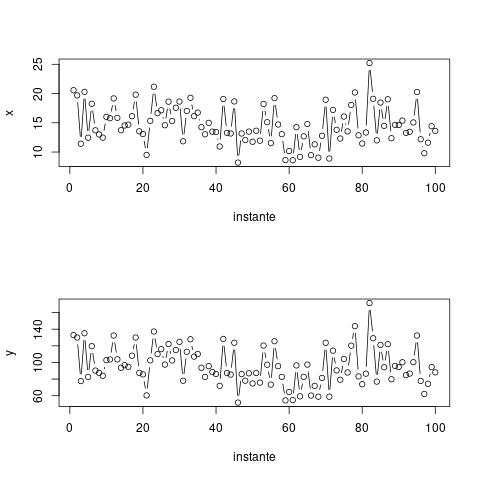
\includegraphics[width=7.5cm]{img/alta_coorelacion.jpeg}
\caption{\(r = 0.9964379\)}
\end{figure}

\pagebreak

\subsection*{Baja correlación (Breast Cancer Wisconsin)}
\label{sec:org817a66d}
Se evaluaron las columnas, 3 (radius) y 4 (textura). la correlación es muy
baja por la textura no afecta a el radio.

\begin{figure}[htbp]
\centering
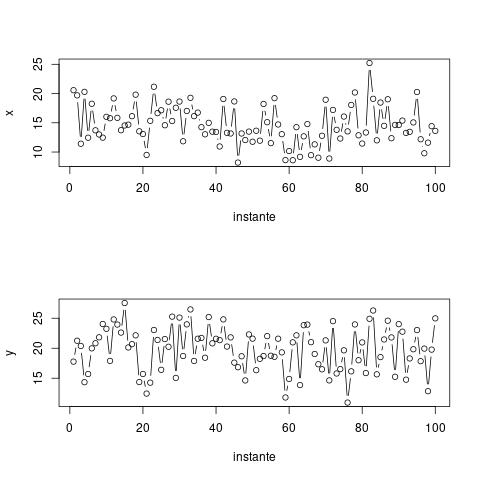
\includegraphics[width=7.5cm]{img/baja_corelacion.jpeg}
\caption{\(r=0.468663\)}
\end{figure}

\subsection*{Correlación Inversa (Real estate valuation data set)}
\label{sec:orgfebecb6}
Se evaluaron las columnas 4 (the number of convenience stores in the living
 circle on foot) y 7 (house price of unit area) por lo que podemos determinar 
que las casa de mayor valor estan lejos de las tiendas.

\begin{figure}[htbp]
\centering
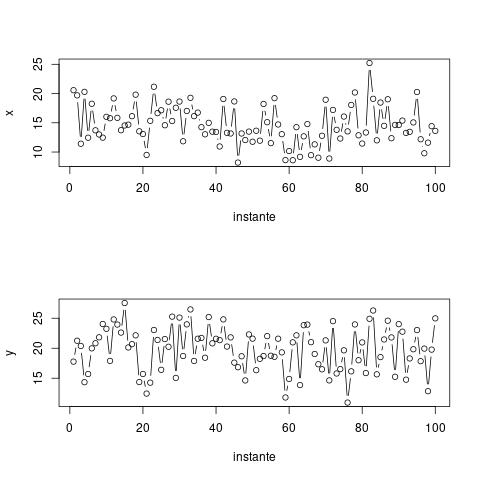
\includegraphics[width=7.5cm]{img/corelacion_inversa.jpeg}
\caption{\(r=-0.8917442\)}
\end{figure}

\section*{Código}
\label{sec:org07241bb}
\lstinputlisting{./src/correlacion.R}
\end{document}
